\documentclass[10pt,a4paper]{article}

% --- Page Geometry & Typography ---
\usepackage[margin=1.9cm]{geometry}
\usepackage[T1]{fontenc}
\usepackage[utf8]{inputenc}
\usepackage{lmodern}
\usepackage{microtype}
\usepackage{graphicx}

% --- Color Palette ---
\usepackage{xcolor}
\definecolor{navy}{HTML}{123047}
\definecolor{teal}{HTML}{007C7A}
\definecolor{sky}{HTML}{DCEFF1}
\definecolor{orange}{HTML}{E67E22}
\definecolor{pale}{HTML}{F8FAFB}
\definecolor{darkgray}{HTML}{333333}
\definecolor{accentblue}{HTML}{1A5276}
\definecolor{lightborder}{HTML}{CBD5E1}

% --- Tables & Arrays ---
\usepackage{booktabs}
\usepackage{tabularx}
\usepackage{array}
\usepackage{longtable}
\renewcommand{\arraystretch}{1.2}
\newcolumntype{Y}{>{\raggedright\sloppy\arraybackslash}X}
\newcolumntype{C}{>{\centering\sloppy\arraybackslash}X}

% --- Mathematics & Symbols ---
\usepackage{amsmath,amssymb}

% --- Lists & Formatting ---
\usepackage{enumitem}
\setlength{\parindent}{1.0em}
\setlength{\parskip}{0.3em}

% --- TikZ & Visual WBS Trees ---
\usepackage{tikz}
\usetikzlibrary{arrows.meta,positioning,calc,fit,shapes.geometric,backgrounds,trees}

\tikzset{
    wbs_root/.style={draw=navy, fill=navy, text=white, font=\bfseries\small, rounded corners=3pt, align=center, inner sep=6pt, minimum width=3.8cm, minimum height=0.9cm},
    wbs_l2/.style={draw=teal, fill=teal!15, text=navy, font=\bfseries\scriptsize, rounded corners=3pt, align=center, inner sep=5pt, minimum width=2.8cm, minimum height=0.8cm},
    wbs_l3/.style={draw=accentblue, fill=sky!40, text=darkgray, font=\scriptsize, rounded corners=2pt, align=center, inner sep=4pt, minimum width=2.4cm},
    wbs_edge/.style={draw=navy!80, -{Latex[length=2mm]}, thick}
}

% --- Citations & Hyperlinks ---
\usepackage{hyperref}
\hypersetup{
    colorlinks=true,
    linkcolor=navy,
    citecolor=teal,
    urlcolor=teal,
    pdftitle={Interface Subsystem Work Breakdown Structure (WBS) - VDI 2206 Engineering Specification},
    pdfauthor={Robotics Mechatronics & Software Systems Team}
}

\begin{document}

% --- Header / Title ---
\begin{center}
    {\LARGE\bfseries\color{navy} Work Breakdown Structure (WBS) Specification\par}
    \vspace{0.4em}
    {\Large\bfseries\color{teal} Domain Allocation \& Work Packages: Interface Software Subsystem\par}
    \vspace{0.5em}
    {\small\textbf{Framework:} VDI 2206 Mechatronic System Design (Descending Branch Phase 2 / ISO 13482 Safety Guidelines)\par}
    \vspace{0.2em}
    {\footnotesize Mechatronics Engineering Graduation Project \quad$\vert$\quad Technical Report WP-SW-04 \quad$\vert$\quad October 2026\par}
\end{center}

\vspace{0.5em}
\hrule height 1.2pt
\vspace{1.0em}

\begin{abstract}
This engineering specification defines the formal Work Breakdown Structure (WBS) for the \textbf{Interface Software Subsystem} (WP-SW-04) of the modular semi-humanoid robotic platform. In compliance with the \textbf{VDI 2206} design methodology for mechatronic and cyber-physical systems (CPS), the software domain is decomposed into six canonical pillars: Navigation (Nav2), Arm Control (MoveIt~2), Machine Vision, Interface, Vision-Language-Action (VLA), and Low-Level Firmware (\texttt{micro\_ros} + \texttt{ros2\_control}). Within this hierarchy, the Interface Subsystem bridges high-level cognitive models, deterministic control middleware, human operators, and distributed edge networks. This document details the Level-2 through Level-4 decomposition of the five interface pillars: \textbf{(1) Browser Teleoperation \& Web Dashboard, (2) Standardized Task Port Gateway, (3) Autonomous Skill Marketplace \& Registry, (4) Physical \& Ambient HMI, and (5) Developer Client SDK \& API Gateways}. For each work package, technical scopes, engineering deliverables, interface contracts, and quantifiable acceptance verification metrics are rigorously formulated.
\end{abstract}

\section{System Context \& VDI 2206 Architectural Integration}
\label{sec:system_context}

In accordance with the \textbf{VDI 2206} V-model for multidisciplinary mechatronic engineering, the system design phase maps functional requirements into decoupled domain-specific components: Mechanical, Electrical/Embedded, and Computer Science/Software. The software domain is structured as a multi-rate, contract-driven architecture that rigorously decouples probabilistic cognition from hard real-time physical control:
\begin{equation}
    \mathcal{S}_{\text{Software}} = \Big\{ \mathcal{D}_{\text{NAV2}}, \ \mathcal{D}_{\text{MoveIt2}}, \ \mathcal{D}_{\text{Vision}}, \ \mathcal{D}_{\text{Interface}}, \ \mathcal{D}_{\text{VLA}}, \ \mathcal{D}_{\text{LowLevel}} \Big\}.
\end{equation}

Within this topology, the \textbf{Interface Subsystem} ($\mathcal{D}_{\text{Interface}}$, designated as \textbf{WBS 4.0}) serves as the mandatory mediator between external agents (human operators, fleet management servers, third-party developers, on-chassis touchpoints) and internal robotic engines. To guarantee absolute compliance with the \textbf{Command Contract} and ISO~13482 personal care robotics safety guidelines, no external interface may directly write to raw actuator registers, motor current loops, or low-level PWM buses. Instead, all interaction flows across validated action servers, projection filters, and sandboxed execution runtimes.

\begin{figure}[htbp]
\centering
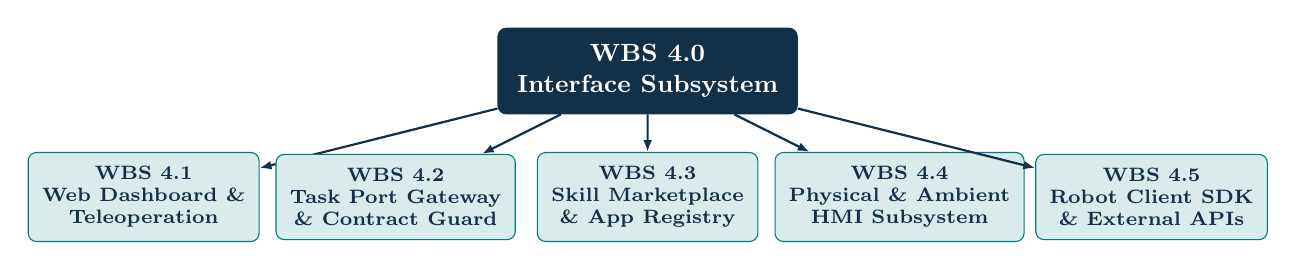
\begin{tikzpicture}[
    level 1/.style={sibling distance=3.2cm, level distance=1.6cm},
    level 2/.style={sibling distance=2.9cm, level distance=1.5cm},
    edge from parent/.style={draw=navy, -{Latex[length=1.5mm]}, thick}
]
\node[wbs_root] {WBS 4.0\\Interface Subsystem}
    child { node[wbs_l2] {WBS 4.1\\Web Dashboard \&\\Teleoperation} }
    child { node[wbs_l2] {WBS 4.2\\Task Port Gateway\\\& Contract Guard} }
    child { node[wbs_l2] {WBS 4.3\\Skill Marketplace\\\& App Registry} }
    child { node[wbs_l2] {WBS 4.4\\Physical \& Ambient\\HMI Subsystem} }
    child { node[wbs_l2] {WBS 4.5\\Robot Client SDK\\\& External APIs} };
\end{tikzpicture}
\caption{Level-2 structural decomposition of the Interface Software Subsystem ($\mathcal{D}_{\text{Interface}}$) under the VDI 2206 framework.}
\label{fig:wbs_tree}
\end{figure}

\section{Hierarchical Work Breakdown Structure (Level 2 to Level 4)}
\label{sec:wbs_decomposition}

The Interface Subsystem is decomposed into 5 Level-2 work elements, 17 Level-3 work packages, and 45 Level-4 discrete engineering work tasks.

% =========================================================================
% WBS 4.1 Web Dashboard
% =========================================================================
\subsection{WBS 4.1: Browser Teleoperation \& Web Fleet Dashboard}
\textbf{Objective:} Provide a zero-install, responsive single-page web console (React / TypeScript / Vite / TailwindCSS) enabling remote situational awareness, glass-to-glass low-latency video streaming, bilateral joystick/gamepad teleoperation, interactive point cloud visualization, and flight telemetry logging.

\begin{itemize}[leftmargin=1.5em]
    \item \textbf{WBS 4.1.1: WebRTC Real-Time Video Streaming Subsystem}
    \begin{itemize}[leftmargin=1.2em]
        \item \emph{4.1.1.1 H.264 GStreamer Hardware Acceleration Pipeline:} Configure Jetson Orin NVENC hardware encoder plugins to capture RealSense stereo RGB-D streams ($1280\times720$ @ 30~fps) with glass-to-glass latency $t_{\text{g2g}} \le 80\text{ ms}$.
        \item \emph{4.1.1.2 WebRTC Signaling \& NAT Traversal Gateway:} Implement WebSocket signaling daemon with STUN/TURN traversal fallback for secure WAN/LAN teleoperation.
        \item \emph{4.1.1.3 Multi-Camera HUD Compositor:} Ingest auxiliary wrist and neck RGB streams into selectable dashboard picture-in-picture (PiP) viewport layouts.
    \end{itemize}

    \item \textbf{WBS 4.1.2: Dual-Protocol Middleware Bridge (WebSocket / Zenoh-Bridge-Web)}
    \begin{itemize}[leftmargin=1.2em]
        \item \emph{4.1.2.1 Rosbridge Suite Integration \& QoS Rate Decimator:} Bridge ROS~2 topics, services, and actions to browser WebSockets with dynamic topic rate throttling (downsampling 100~Hz state topics to 20~Hz browser updates to conserve network bandwidth).
        \item \emph{4.1.2.2 Zenoh-Bridge-Web Ultra-Low Latency Transport:} Provide native WebAssembly (Wasm) Zenoh client bindings for peer-to-peer telemetry streaming bypassing JSON serialization overhead.
        \item \emph{4.1.2.3 Token-Based Authentication \& RBAC Interceptor:} Enforce JWT/mTLS token authorization for teleoperator session establishment and operator privilege escalation.
    \end{itemize}

    \item \textbf{WBS 4.1.3: Teleoperation \& Input Controller Layer}
    \begin{itemize}[leftmargin=1.2em]
        \item \emph{4.1.3.1 HTML5 Gamepad API Driver:} Support dual-analog industrial/consumer gamepads (e.g., Logitech F710, Xbox) with deadband calibration, exponential throttle curves, and button mapping profiles.
        \item \emph{4.1.3.2 Virtual Touch Joysticks \& Mobile Responsive UI:} Render touch-sensitive on-screen virtual joysticks for tablet/smartphone operation with emergency release deadman switch.
        \item \emph{4.1.3.3 End-Effector Cartesian Jogging Console:} Interactive 6-DoF Cartesian jog widgets for incremental millimeter-precision tool-flange positioning and tool orientation adjustments.
    \end{itemize}

    \item \textbf{WBS 4.1.4: 3D Digital Twin \& Sensor Data Visualization}
    \begin{itemize}[leftmargin=1.2em]
        \item \emph{4.1.4.1 Three.js / WebGL URDF Robot Model Renderer:} Real-time 3D synchronized rendering of the 18-DoF robot kinematic chain driven by live \texttt{/joint\_states} topic transforms.
        \item \emph{4.1.4.2 2D LiDAR Costmap \& Nav2 Goal Pose Interactor:} Stream 2D occupancy grids and local costmaps with click-and-drag interactive navigation goal and orientation placement tools.
        \item \emph{4.1.4.3 Point Cloud Downsampler \& Octree Visualizer:} WebGL point cloud shader visualizing RealSense 3D point clusters with client-side voxel downsampling ($<150\text{k}$ points/frame).
    \end{itemize}

    \item \textbf{WBS 4.1.5: System Health, Telemetry \& Flight Recorder Dashboard}
    \begin{itemize}[leftmargin=1.2em]
        \item \emph{4.1.5.1 Power Domain \& Battery BMS Gauge Console:} Real-time visual display of cell voltages, State of Charge ($\text{SoC}\%$), power draw (W), and thermal status across the 24V, 19V, 12V, and 5V rails.
        \item \emph{4.1.5.2 Motor Actuator Diagnostic Matrix:} Grid monitor for all 9$\times$ CubeMars AK70-10 QDDs and 6$\times$ Feetech servos showing winding temperature, phase current, bus voltage, and error flags.
        \item \emph{4.1.5.3 ROS 2 Node Lifecycle Inspector \& Diagnostic Logger:} Interactive console visualizing ROS~2 Lifecycle Node transitions, active fault logs, and historical diagnostic bag downloads.
    \end{itemize}
\end{itemize}

% =========================================================================
% WBS 4.2 Task Port Gateway
% =========================================================================
\subsection{WBS 4.2: Standardized Task Port Gateway \& Contract Guard}
\textbf{Objective:} Provide a strictly typed, versioned ROS~2 Action and Service gateway that isolates low-level real-time controllers from external cognitive models and users, enforcing the mathematical Command Contract and ISO~13482 safety envelope.

\begin{itemize}[leftmargin=1.5em]
    \item \textbf{WBS 4.2.1: High-Level Primitive Action Server Implementations}
    \begin{itemize}[leftmargin=1.2em]
        \item \emph{4.2.1.1 Navigation Task Port (\texttt{/navigate\_to\_pose}):} Wrap Nav2 navigation client into an observable action interface supporting goal preemption, obstacle wait timeouts, and dynamic recovery behaviors.
        \item \emph{4.2.1.2 Tabletop Manipulation Task Port (\texttt{/pick\_object}, \texttt{/place\_object}):} Expose semantic object pick/place primitives accepting detected object bounding boxes, automatically generating grasp poses, pre-approach trajectories, and compliant grip triggers.
        \item \emph{4.2.1.3 Autonomous Docking Task Port (\texttt{/dock\_robot}):} Closed-loop docking primitive aligning with charging contacts via infrared and LiDAR retro-reflector feedback.
        \item \emph{4.2.1.4 Bimanual Coordinated Carry Task Port (\texttt{/carry\_dual\_arm}):} Synchronous dual-arm Cartesian action enforcing closed kinematic chain constraints during payload transport.
    \end{itemize}

    \item \textbf{WBS 4.2.2: Mathematical Command Contract Verification \& Projection Filter}
    \begin{itemize}[leftmargin=1.2em]
        \item \emph{4.2.2.1 Feasible Set Projector ($\Pi_{\mathcal{F}}$ Operator):} Quadratic programming solver projecting incoming external trajectory deltas into the verified feasible space $\mathcal{F}(\mathbf{q}, \mathcal{E}, \mathcal{S})$, clamping velocities, accelerations, and workspace boundaries.
        \item \emph{4.2.2.2 Observable Safety Projection Veto Engine:} Continuous residual monitoring ($\varepsilon_{\text{proj}} > \varepsilon_{\text{tol}}$). Automatically veto unsafe AI proposals, emit structured \texttt{SafetyVeto} warnings, and trigger smooth kinematic deceleration stops within $\le 20\text{ ms}$.
        \item \emph{4.2.2.3 ISO 13482 Dynamic Speed \& Separation Monitor (SSM):} Dynamically scale max tool and base velocity inversely with human proximity detected via 2D LiDAR and depth camera fields.
    \end{itemize}

    \item \textbf{WBS 4.2.3: Task State Machine \& Execution Supervisor}
    \begin{itemize}[leftmargin=1.2em]
        \item \emph{4.2.3.1 BehaviorTree.CPP Execution Root Bridge:} Translate incoming Task Port action goals into parameterized Behavior Tree blackboard variables and supervise tree ticking lifecycle.
        \item \emph{4.2.3.2 Preemption, Cancellation \& Pause Handler:} Deterministic cancellation handler safely transitioning manipulators and base to locked stationary states upon operator override or external preemption.
        \item \emph{4.2.3.3 Structured Failure Diagnostic Code Generator:} Output standardized error classification schemas (e.g., \texttt{ERR\_IK\_UNREACHABLE}, \texttt{ERR\_PATH\_BLOCKED}, \texttt{ERR\_GRASP\_SLIP}) for automated upstream replanning.
    \end{itemize}
\end{itemize}

% =========================================================================
% WBS 4.3 Skill Marketplace & App Registry
% =========================================================================
\subsection{WBS 4.3: Autonomous Skill Marketplace \& Application Registry}
\textbf{Objective:} Provide a modular, secure runtime repository and lifecycle orchestrator for packaging, distributing, dynamically loading, and executing modular robot skills, AI policies, and composite behavior trees without recompiling system software.

\begin{itemize}[leftmargin=1.5em]
    \item \textbf{WBS 4.3.1: Standardized Robot Skill Packaging Format}
    \begin{itemize}[leftmargin=1.2em]
        \item \emph{4.3.1.1 Skill Package Schema Definition (OpenUSD / JSON-Schema):} Manifest specification declaring skill entry points, input/output parameters, required hardware interfaces, pre/post-conditions, and execution safety envelopes.
        \item \emph{4.3.1.2 Deterministic Behavior Tree XML Bundler:} Containerized packaging of BehaviorTree.CPP XML subtrees, node plugins, and associated ROS~2 parameter YAML configurations.
        \item \emph{4.3.1.3 Policy Checkpoint \& Neural Weight Artifactory:} Standardized storage format for ONNX/TensorRT policy weights (e.g., OpenVLA affordance chunks, tactile slip models) with SHA-256 integrity verification.
    \end{itemize}

    \item \textbf{WBS 4.3.2: On-Robot Skill Engine \& Dynamic Plugin Loader}
    \begin{itemize}[leftmargin=1.2em]
        \item \emph{4.3.2.1 Shared Library PluginLoader Service:} Dynamic runtime loading and unloading of compiled C++ BehaviorTree action nodes and MoveIt planning plugins without restarting core ROS~2 daemons.
        \item \emph{4.3.2.2 Skill Dependency Validator \& Capability Checker:} Pre-flight introspection verifying that required sensors, joint limits, end-effectors, and transform frames are online and calibrated before initiating execution.
        \item \emph{4.3.2.3 Sandboxed Execution Environment:} Micro-container / cgroups process jail isolating experimental third-party skills, enforcing CPU, memory, and bus bandwidth quotas.
    \end{itemize}

    \item \textbf{WBS 4.3.3: Marketplace Cloud / Local Registry \& Package Manager}
    \begin{itemize}[leftmargin=1.2em]
        \item \emph{4.3.3.1 Local Skill Repository Web UI:} Web Dashboard catalog view allowing operators to search, browse, install, inspect parameters, and execute installed platform skills.
        \item \emph{4.3.3.2 Cloud Sync \& Over-The-Air (OTA) Release Client:} Secure HTTPS/gRPC client synchronizing approved enterprise skill bundles, verified firmware revisions, and cryptographic license tokens.
        \item \emph{4.3.3.3 Graphical Behavior Tree Macro Composer:} Web-based visual drag-and-drop workflow editor enabling users to chain discrete skills into custom sequential and parallel mission trees.
    \end{itemize}
\end{itemize}

% =========================================================================
% WBS 4.4 Physical & Ambient HMI Subsystem
% =========================================================================
\subsection{WBS 4.4: Physical, Acoustic \& Ambient HMI Subsystem}
\textbf{Objective:} Implement the multimodal physical human-robot interface on the robot body, including the torso touchscreen GUI, ambient expression LED indicator, directional speech synthesis/recognition, and hardware service bulkhead.

\begin{itemize}[leftmargin=1.5em]
    \item \textbf{WBS 4.4.1: Torso Embedded Touchscreen GUI (Kiosk Mode)}
    \begin{itemize}[leftmargin=1.2em]
        \item \emph{4.4.1.1 Lightweight On-Chassis UI (Flutter / Qt Embedded):} 5--7'' touch display application running in kiosk mode with high-contrast outdoor/indoor UI themes and glove-friendly touch targets.
        \item \emph{4.4.1.2 Quick-Diagnostic \& Network Configuration View:} Immediate display of IP addresses, Wi-Fi connectivity wizard, battery SoC\%, hardware temperature readouts, and E-Stop latch status.
        \item \emph{4.4.1.3 On-Site Pin-Protected Task Dispatcher:} Local interface enabling facility workers to select and dispatch predefined local routines (e.g., ``Go to Cleaning Bay'', ``Handover Parcel'') without requiring a laptop.
    \end{itemize}

    \item \textbf{WBS 4.4.2: Expressive Ambient Lighting \& Head Audio HMI}
    \begin{itemize}[leftmargin=1.2em]
        \item \emph{4.4.2.1 Addressable RGB LED Ring Controller:} ESP32-driven WS2812B NeoPixel ring mounted on the head perimeter displaying unambiguous system states (e.g., solid green: idle ready; pulsing blue: autonomous motion; blinking amber: obstacle pause; flashing red: E-Stop).
        \item \emph{4.4.2.2 Directional Audio \& Head Gaze Tracker:} Coordinate ReSpeaker dual-mic array TDOA sound localization with the 2-DoF pan/tilt neck servos, autonomously turning the robot head toward an interacting human speaker.
        \item \emph{4.4.2.3 Text-To-Speech (TTS) \& Acoustic Feedback Daemon:} Onboard Piper/VITS neural speech synthesizer generating low-latency ($<200\text{ ms}$) natural voice confirmations and audible safety alarm chimes over the 2W internal speaker.
    \end{itemize}

    \item \textbf{WBS 4.4.3: Physical Bulkhead Service Bay \& Mechanical HMI}
    \begin{itemize}[leftmargin=1.2em]
        \item \emph{4.4.3.1 Hardware Interlock \& E-Stop UI Monitoring:} Sense NC loop contacts of the torso mushroom E-Stop button and report trip timestamp and circuit resistance via digital GPIO optocouplers.
        \item \emph{4.4.3.2 Bulkhead USB/RJ45 Maintenance Daemon:} Automatically detect maintenance cable plug-in on the torso service bulkhead, spawning isolated tethered development networks and auto-mounting diagnostic flash media.
    \end{itemize}
\end{itemize}

% =========================================================================
% WBS 4.5 Developer Client SDK & External APIs
% =========================================================================
\subsection{WBS 4.5: Developer Client SDK \& External Integration Gateways}
\textbf{Objective:} Provide native client libraries, RESTful/WebSocket APIs, and industrial fleet adapters (VDA 5050 / MQTT) to enable seamless third-party software integration, academic research scripting, and warehouse management integration.

\begin{itemize}[leftmargin=1.5em]
    \item \textbf{WBS 4.5.1: High-Level Python Client SDK (\texttt{robot\_sdk})}
    \begin{itemize}[leftmargin=1.2em]
        \item \emph{4.5.1.1 Ergonomic Python Asynchronous API:} Provide intuitive Pythonic classes (\texttt{Robot}, \texttt{Arm}, \texttt{Base}, \texttt{Gripper}, \texttt{Head}) wrapping complex ROS~2 actions into \texttt{asyncio} Python promises.
        \item \emph{4.5.1.2 Kinematics \& Transform Client Utilities:} Local client-side forward kinematics helpers, coordinate frame transforms ($SE(3)$ representations), and spatial vector math utilities.
        \item \emph{4.5.1.3 Demonstration Recording \& Replay Toolkit:} CLI tool to record synchronous streams of joint positions, gripper states, and RGB-D images into HDF5/Zarr formats for imitation learning and dataset curation.
    \end{itemize}

    \item \textbf{WBS 4.5.2: RESTful \& WebSocket API Gateway Server}
    \begin{itemize}[leftmargin=1.2em]
        \item \emph{4.5.2.1 OpenAPI / Swagger REST Endpoints (FastAPI):} Asynchronous HTTP gateway exposing system status, telemetry queries, skill listings, configuration updates, and mission dispatching for web developers.
        \item \emph{4.5.2.2 Push-Event WebSocket Telemetry Streamer:} High-throughput JSON/MessagePack event stream pushing asynchronous state changes, battery events, and task completion notices to subscribed client applications.
        \item \emph{4.5.2.3 Security Gateway (OAuth2 / TLS 1.3 Encryption):} Strict end-to-end cryptographic encryption with API key generation, rate limiting, and automated certificate renewal.
    \end{itemize}

    \item \textbf{WBS 4.5.3: Industrial Enterprise \& Logistics Adapters}
    \begin{itemize}[leftmargin=1.2em]
        \item \emph{4.5.3.1 VDA 5050 Fleet Interface Adapter:} Native translation bridge converting AGV/AMR standard VDA~5050 order topics and instant actions into Nav2 goal dispatches and state telemetry reports.
        \item \emph{4.5.3.2 Industrial MQTT IoT Bridge:} Lightweight telemetry publishing client transmitting machine operating hours, energy consumption, and fault indicators to factory IoT brokers.
    \end{itemize}
\end{itemize}

\section{Work Package Specification \& Allocation Matrix}
\label{sec:allocation_matrix}

Table~\ref{tab:interface_wbs_matrix} formalizes the engineering allocation matrix for the Interface Subsystem in strict compliance with the project's VDI 2206 requirements, identifying responsible engineering sub-disciplines, explicit work package deliverables, cross-domain interface boundaries, and quantifiable verification criteria.

\begin{small}
\begin{longtable}{@{}p{0.10\textwidth} p{0.22\textwidth} p{0.24\textwidth} p{0.24\textwidth} p{0.14\textwidth}@{}}
\caption{VDI 2206 engineering work package allocation matrix for Interface Software Subsystem (WP-SW-04).}
\label{tab:interface_wbs_matrix}\\
\toprule
\textbf{WBS Code} & \textbf{Work Package Title} & \textbf{Scope \& Key Responsibilities} & \textbf{Primary Deliverables} & \textbf{Verification Metric} \\
\midrule
\endfirsthead
\multicolumn{5}{c}{{\bfseries Table \thetable\ continued from previous page}} \\
\toprule
\textbf{WBS Code} & \textbf{Work Package Title} & \textbf{Scope \& Key Responsibilities} & \textbf{Primary Deliverables} & \textbf{Verification Metric} \\
\midrule
\endhead
\midrule
\multicolumn{5}{r}{{Continued on next page\dots}} \\
\bottomrule
\endfoot
\bottomrule
\endlastfoot

\textbf{4.1.1} & 
WebRTC Video Teleop Pipeline & 
GStreamer NVENC hardware encoding of RealSense color/depth streams, WebRTC signaling server, NAT traversal. & 
C++ ROS~2 WebRTC streamer node, signaling daemon, browser video client component. & 
Glass-to-glass latency $t_{\text{g2g}} \le 80\text{ ms}$; frame rate $\ge 30\text{ fps}$ at $720\text{p}$; CPU load $<10\%$. \\
\addlinespace[3pt]

\textbf{4.1.2} & 
WebSocket / Zenoh Bridge & 
Two-way state telemetry transport, dynamic topic decimation, JWT token authentication, client session handling. & 
Rosbridge configuration packages, Zenoh-Web Wasm module, auth middleware plugin. & 
Telemetry rate $\ge 20\text{ Hz}$; round-trip command latency $\le 25\text{ ms}$; zero unauthorized packet leaks. \\
\addlinespace[3pt]

\textbf{4.1.3} & 
Gamepad \& Jogging Layer & 
HTML5 gamepad input mapping, deadband compensation, mobile touch joysticks, 6-DoF Cartesian jog widgets. & 
React controller hooks, virtual joystick UI component, Cartesian jog action client. & 
Input dispatch jitter $<5\text{ ms}$; deadman disconnect stop latency $\le 50\text{ ms}$. \\
\addlinespace[3pt]

\textbf{4.1.4} & 
3D Digital Twin Visualizer & 
Three.js URDF model rendering, live TF frame synchronization, 2D Nav2 costmap overlay, point cloud shaders. & 
WebGL canvas component, TF tree subscriber, point cloud downsampling worker. & 
Render frame rate $\ge 60\text{ fps}$; point cloud capacity $\ge 150\text{k}$ points; transform error $0\text{ mm}$. \\
\addlinespace[3pt]

\textbf{4.1.5} & 
Diagnostics \& Flight Logger & 
Power rail BMS telemetry display, motor actuator thermal/current gauges, ROS~2 node lifecycle dashboard. & 
Diagnostic dashboard UI, real-time alert toast notification system, bag exporter. & 
Update latency $\le 100\text{ ms}$; $100\%$ fault coverage across all 15 active actuators. \\
\midrule

\textbf{4.2.1} & 
Primitive Task Action Servers & 
High-level action interfaces for navigation, tabletop pick/place, autonomous docking, and bimanual carry. & 
ROS~2 Action packages (\texttt{NavigateToPose}, \texttt{PickObject}, \texttt{Dock}), client test suites. & 
Action dispatch latency $\le 25\text{ ms}$; preemption reaction time $\le 15\text{ ms}$; $100\%$ parameter typing. \\
\addlinespace[3pt]

\textbf{4.2.2} & 
Command Contract Guard & 
$\Pi_{\mathcal{F}}$ quadratic projection operator, velocity/acceleration clamping, safety veto handler, ISO 13482 SSM. & 
C++ real-time lifecycle guard node, projection optimization library, unit test harness. & 
Projection solve time $\le 2\text{ ms}$; safety veto trigger time $\le 20\text{ ms}$; zero unprojected writes. \\
\addlinespace[3pt]

\textbf{4.2.3} & 
Task Execution Supervisor & 
BehaviorTree.CPP engine wrapper, blackboard variable injection, preemption/pause handlers, error code schemas. & 
BT execution engine package, lifecycle supervisor node, structured error definition headers. & 
State transition deterministic latency $<5\text{ ms}$; zero deadlocks on sub-tree aborts. \\
\midrule

\textbf{4.3.1} & 
Skill Packaging Format & 
Specification of skill schema, BehaviorTree XML packaging, ONNX/TensorRT model weight artifactory. & 
Skill manifest JSON schema, packaging CLI tool (\texttt{skill-pack}), verification test suites. & 
Schema validation time $<50\text{ ms}$; cryptographic hash verification $100\%$ tamper-proof. \\
\addlinespace[3pt]

\textbf{4.3.2} & 
Dynamic Plugin Loader & 
Runtime C++ plugin loading via \texttt{pluginlib}, pre-flight hardware dependency checker, sandboxed cgroups jail. & 
Dynamic skill runner node, pre-flight inspection script, cgroups isolation configuration. & 
Plugin load time $<500\text{ ms}$; zero core daemon crashes upon bad plugin abort. \\
\addlinespace[3pt]

\textbf{4.3.3} & 
Marketplace \& Composer & 
Local skill catalog UI, cloud sync client, visual drag-and-drop Behavior Tree composer. & 
Marketplace web application, OTA sync client daemon, graphical web node editor. & 
UI tree compilation to valid XML $<100\text{ ms}$; OTA rollback capability $\le 10\text{ s}$. \\
\midrule

\textbf{4.4.1} & 
Torso Touchscreen Kiosk & 
5--7'' touch display UI in kiosk mode, network config wizard, battery/error monitor, local task trigger. & 
Touchscreen UI application (Flutter/Qt), systemd kiosk service, pin authentication module. & 
Cold boot to touch response $\le 8\text{ s}$; UI frame rate $\ge 60\text{ fps}$; touch latency $<30\text{ ms}$. \\
\addlinespace[3pt]

\textbf{4.4.2} & 
Expressive Lighting \& Audio & 
WS2812B NeoPixel ring state animations, ReSpeaker TDOA head gaze tracking, Piper neural TTS voice synthesizer. & 
ESP32 LED firmware, head gaze tracking node, local TTS audio generation service. & 
Sound localization angle accuracy $\pm 10^\circ$; gaze tracking response $<300\text{ ms}$; TTS latency $<200\text{ ms}$. \\
\addlinespace[3pt]

\textbf{4.4.3} & 
Physical Bulkhead Bay & 
Hardware E-Stop status sensing via optocouplers, bulkhead USB/GbE automatic network tether daemon. & 
Optocoupler sensing driver, auto-tether udev scripts, maintenance terminal launcher. & 
E-Stop state detection latency $\le 5\text{ ms}$; tether network acquisition time $<3.0\text{ s}$. \\
\midrule

\textbf{4.5.1} & 
Python Client SDK & 
Async Python library wrapping Task Port actions, kinematics utilities, HDF5 demonstration recording tools. & 
\texttt{robot\_sdk} Python package (wheel), Sphinx documentation, developer code examples. & 
API documentation test coverage $\ge 90\%$; action dispatch round-trip $<10\text{ ms}$. \\
\addlinespace[3pt]

\textbf{4.5.2} & 
REST \& WebSocket Gateway & 
FastAPI REST endpoints for fleet queries, push-event WebSocket telemetry server, OAuth2 authentication. & 
FastAPI gateway service container, OpenAPI Swagger UI, JWT security layer. & 
REST endpoint response time $t_{99} < 15\text{ ms}$; concurrent WebSocket connections $\ge 50$. \\
\addlinespace[3pt]

\textbf{4.5.3} & 
Industrial Logistics Adapters & 
VDA 5050 AGV/AMR protocol translator, industrial MQTT broker bridge for factory IoT telemetry. & 
VDA 5050 ROS~2 node, MQTT publisher gateway, integration test harness. & 
VDA 5050 compliance certified; message translation latency $<10\text{ ms}$; zero message drops. \\

\end{longtable}
\end{small}

\section{Cross-Subsystem Interface Boundaries \& Data Contracts}
\label{sec:interfaces}

To avoid integration failure modes during Phase~3 of the VDI~2206 model (System Integration), all boundaries between the Interface Subsystem and adjacent subsystems are governed by immutable data contracts:

\begin{figure}[htbp]
\centering
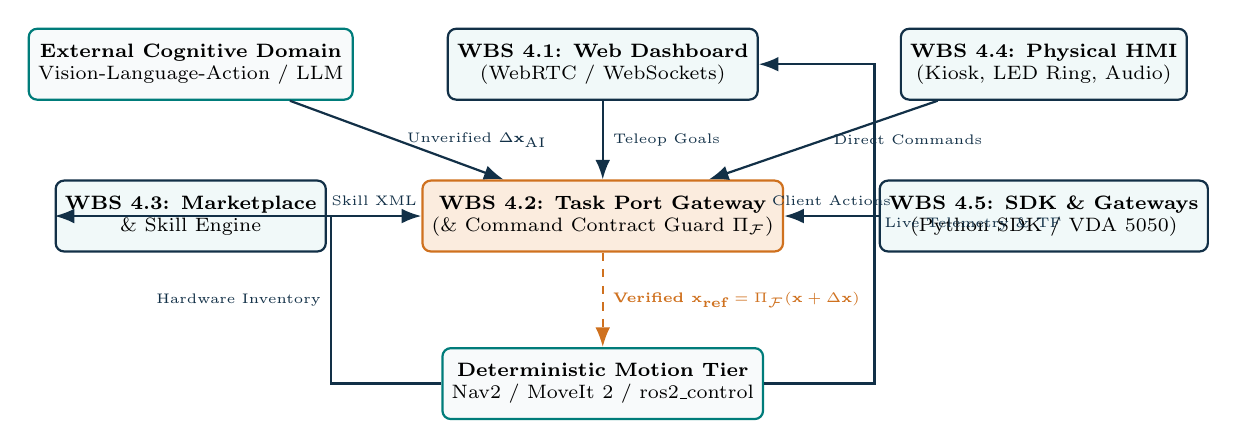
\begin{tikzpicture}[
    node distance=0.8cm and 1.2cm,
    >=Latex,
    every node/.style={font=\scriptsize, align=center},
    int_box/.style={draw=navy, fill=sky!40, rounded corners=3pt, thick, minimum width=3.2cm, minimum height=0.9cm},
    ext_box/.style={draw=teal, fill=pale, rounded corners=3pt, thick, minimum width=3.0cm, minimum height=0.9cm},
    guard_box/.style={draw=orange!90!black, fill=orange!15, rounded corners=3pt, thick, minimum width=3.4cm, minimum height=0.9cm},
    data_flow/.style={-{Latex[length=2.5mm]}, thick, navy},
    safe_flow/.style={-{Latex[length=2.5mm]}, thick, orange!90!black, dashed}
]

  % Core Interface Nodes
  \node[int_box] (dashboard) {\textbf{WBS 4.1: Web Dashboard}\\(WebRTC / WebSockets)};
  \node[guard_box, below=1.0cm of dashboard] (task_port) {\textbf{WBS 4.2: Task Port Gateway}\\(\& Command Contract Guard $\Pi_{\mathcal{F}}$)};
  \node[int_box, left=1.2cm of task_port] (marketplace) {\textbf{WBS 4.3: Marketplace}\\\& Skill Engine};
  \node[int_box, right=1.2cm of task_port] (sdk_api) {\textbf{WBS 4.5: SDK \& Gateways}\\(Python SDK / VDA 5050)};
  \node[int_box, above=1.0cm of sdk_api] (hmi_phys) {\textbf{WBS 4.4: Physical HMI}\\(Kiosk, LED Ring, Audio)};

  % External Subsystem Nodes
  \node[ext_box, above=1.0cm of marketplace] (vla_node) {\textbf{External Cognitive Domain}\\Vision-Language-Action / LLM};
  \node[ext_box, below=1.2cm of task_port] (rt_ctrl) {\textbf{Deterministic Motion Tier}\\Nav2 / MoveIt 2 / ros2\_control};

  % Connecting Flows
  \draw[data_flow] (dashboard) -- node[right, font=\tiny]{Teleop Goals} (task_port);
  \draw[data_flow] (vla_node) -- node[right, font=\tiny]{Unverified $\Delta\mathbf{x}_{\text{AI}}$} (task_port);
  \draw[data_flow] (marketplace) -- node[above, font=\tiny]{Skill XML} (task_port);
  \draw[data_flow] (sdk_api) -- node[above, font=\tiny]{Client Actions} (task_port);
  \draw[data_flow] (hmi_phys) -- node[right, font=\tiny]{Direct Commands} (task_port);

  \draw[safe_flow] (task_port) -- node[right, font=\tiny\bfseries]{Verified $\mathbf{x}_{\text{ref}} = \Pi_{\mathcal{F}}(\mathbf{x}+\Delta\mathbf{x})$} (rt_ctrl);
  \draw[data_flow] (rt_ctrl.east) -- ++(1.4,0) |- node[pos=0.25, right, font=\tiny]{Live Telemetry \& TF} (dashboard.east);
  \draw[data_flow] (rt_ctrl.west) -- ++(-1.4,0) |- node[pos=0.25, left, font=\tiny]{Hardware Inventory} (marketplace.west);

\end{tikzpicture}
\caption{Cross-subsystem data communication and contract enforcement topology.}
\label{fig:interface_topology}
\end{figure}

\begin{enumerate}[leftmargin=1.5em]
    \item \textbf{Interface 4-A (Interface $\to$ Motion Planning [Nav2 / MoveIt 2]):}
    All spatial trajectory and waypoint goals are committed exclusively via ROS~2 action protocols (\texttt{nav2\_msgs/action/NavigateToPose}, \texttt{moveit\_msgs/action/MoveGroup}). The Command Contract Guard guarantees that target goal poses reside within collision-free configuration space prior to planner invocation.
    
    \item \textbf{Interface 4-B (Interface $\to$ Machine Vision \& Perception):}
    High-bandwidth sensory streams (uncompressed $1280\times720$ RGB-D frames, segmented point clouds) are consumed via zero-copy shared memory transports (\texttt{sensor\_msgs/Image}, \texttt{sensor\_msgs/PointCloud2}). The WebRTC pipeline taps into hardware NVENC encoders directly without burdening the host CPU.

    \item \textbf{Interface 4-C (Interface $\to$ Low-Level Firmware [\texttt{micro\_ros} + \texttt{ros2\_control}]):}
    Bidirectional exchange of raw actuator states and commanded joint efforts. Interface 4.1 reads diagnostic registers (winding temperature, current draw, encoder health) across \texttt{diagnostic\_msgs/DiagnosticArray} topics at 10~Hz, completely isolated from the 1~kHz real-time fieldbus loop.

    \item \textbf{Interface 4-D (Interface $\to$ VLA Foundation Policy Domain):}
    The VLA inference policy dispatches proposed spatial deltas $\Delta\mathbf{x}_{\text{AI}}$ via the \texttt{/vla/propose\_action} service. The Task Port Gateway intercepts this unverified vector, subjects it to the quadratic projection $\Pi_{\mathcal{F}}$, and passes only bounded setpoints downstream.
\end{enumerate}

\section{Verification, Testing \& Acceptance Roadmap}
\label{sec:verification}

In adherence to the ascending branch of the VDI~2206 V-model, verification proceeds through three sequential testing gates prior to operational deployment:

\begin{itemize}[leftmargin=1.5em]
    \item \textbf{Gate 1: Software-in-the-Loop (SIL) Virtual Validation:}
    The entire Interface Subsystem is deployed inside containerized Docker environments interfaced to an NVIDIA Isaac Sim / Gazebo physics simulation. Automated CI/CD test suites inject synthetic network degradation (packet dropouts up to $15\%$, latency jitter up to $150\text{ ms}$) to verify WebRTC reconnection robustness, action cancellation determinism, and zero UI crash occurrences.
    
    \item \textbf{Gate 2: Hardware-in-the-Loop (HIL) Testbench Validation:}
    The interface components are deployed onto the physical NVIDIA Jetson Orin NX compute module paired with the physical Torso Touchscreen and ReSpeaker audio head. Bench testing verifies that glass-to-glass video latency remains strictly $\le 80\text{ ms}$, CPU utilization remains below $15\%$, and sound localization accuracy achieves $\pm 10^\circ$.
    
    \item \textbf{Gate 3: Full Platform Integrated Safety \& ISO 13482 Validation:}
    On the integrated mobile manipulator, physical hazard injection tests are performed: triggering manual E-Stop while teleoperating, simulating sudden obstacle occlusion during waypoint jogging, and injecting out-of-bounds trajectory proposals from the VLA model. Acceptance requires that the safety projection veto clamps the command within $\le 20\text{ ms}$ and brings the platform to a controlled stop without mechanical stress.
\end{itemize}

\section{Conclusion}
The Work Breakdown Structure developed herein establishes an exhaustive, mathematically grounded, and modular engineering specification for the Interface Software Subsystem ($\mathcal{D}_{\text{Interface}}$). By decomposing the interface into five decoupled pillars—Web Dashboard, Task Port Gateway, Skill Marketplace, Physical HMI, and Developer SDK—the platform satisfies the functional requirements of modern semi-humanoid robotics: agile teleoperation, secure cognitive AI integration, intuitive human collaboration, and enterprise scalability, while maintaining an uncompromising commitment to ISO~13482 physical safety.

\end{document}
